\documentclass[12pt]{article}

\usepackage{amsmath, amsthm}
\newtheorem{prob}{Problem}
\usepackage{graphicx}
\usepackage{fullpage}

\begin{document}
% begin problem: imo-2010-4 --lang en
\begin{prob}[IMO 2010/4]
Let $P$ be a point interior to triangle $ABC$ (with $CA \neq CB$).
The lines $AP$, $BP$ and $CP$ meet again its circumcircle $\Gamma$ at $K$, $L$, respectively $M$.
The tangent line at $C$ to $\Gamma$ meets the line $AB$ at $S$.
Show that from $SC = SP$ follows $MK = ML$.
\end{prob}
% end problem

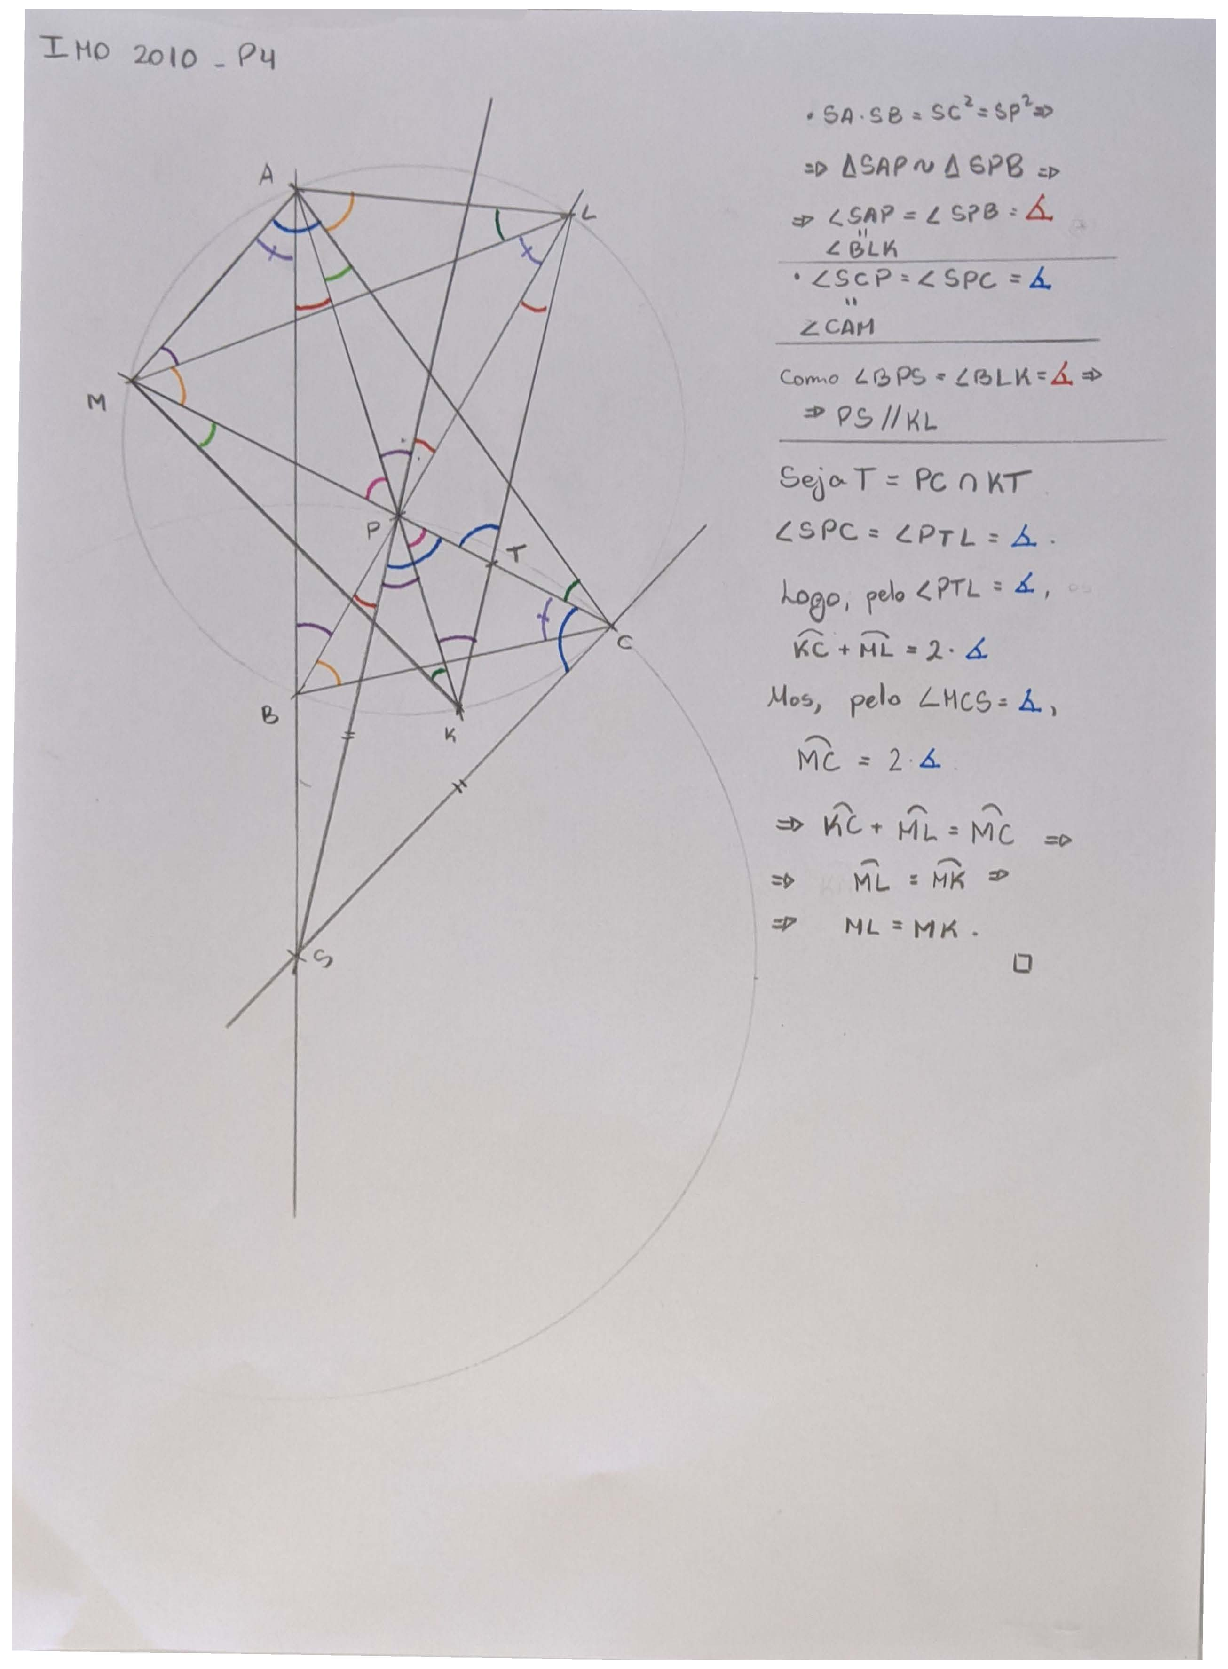
\includegraphics[width = 14cm]{/home/zeus/Documents/solutions/imo-2010-4.pdf}

\newpage

% begin problem: imo-2009-2 --lang en
\begin{prob}[IMO 2009/2]
Let $ ABC$ be a triangle with circumcentre $ O$. The points $ P$ and $ Q$ are interior points of the sides $ CA$ and $ AB$ respectively. Let $ K,L$ and $ M$ be the midpoints of the segments $ BP,CQ$ and $ PQ$. respectively, and let $ \Gamma$ be the circle passing through $ K,L$ and $ M$. Suppose that the line $ PQ$ is tangent to the circle $ \Gamma$. Prove that $ OP = OQ.$
\end{prob}
% end problem

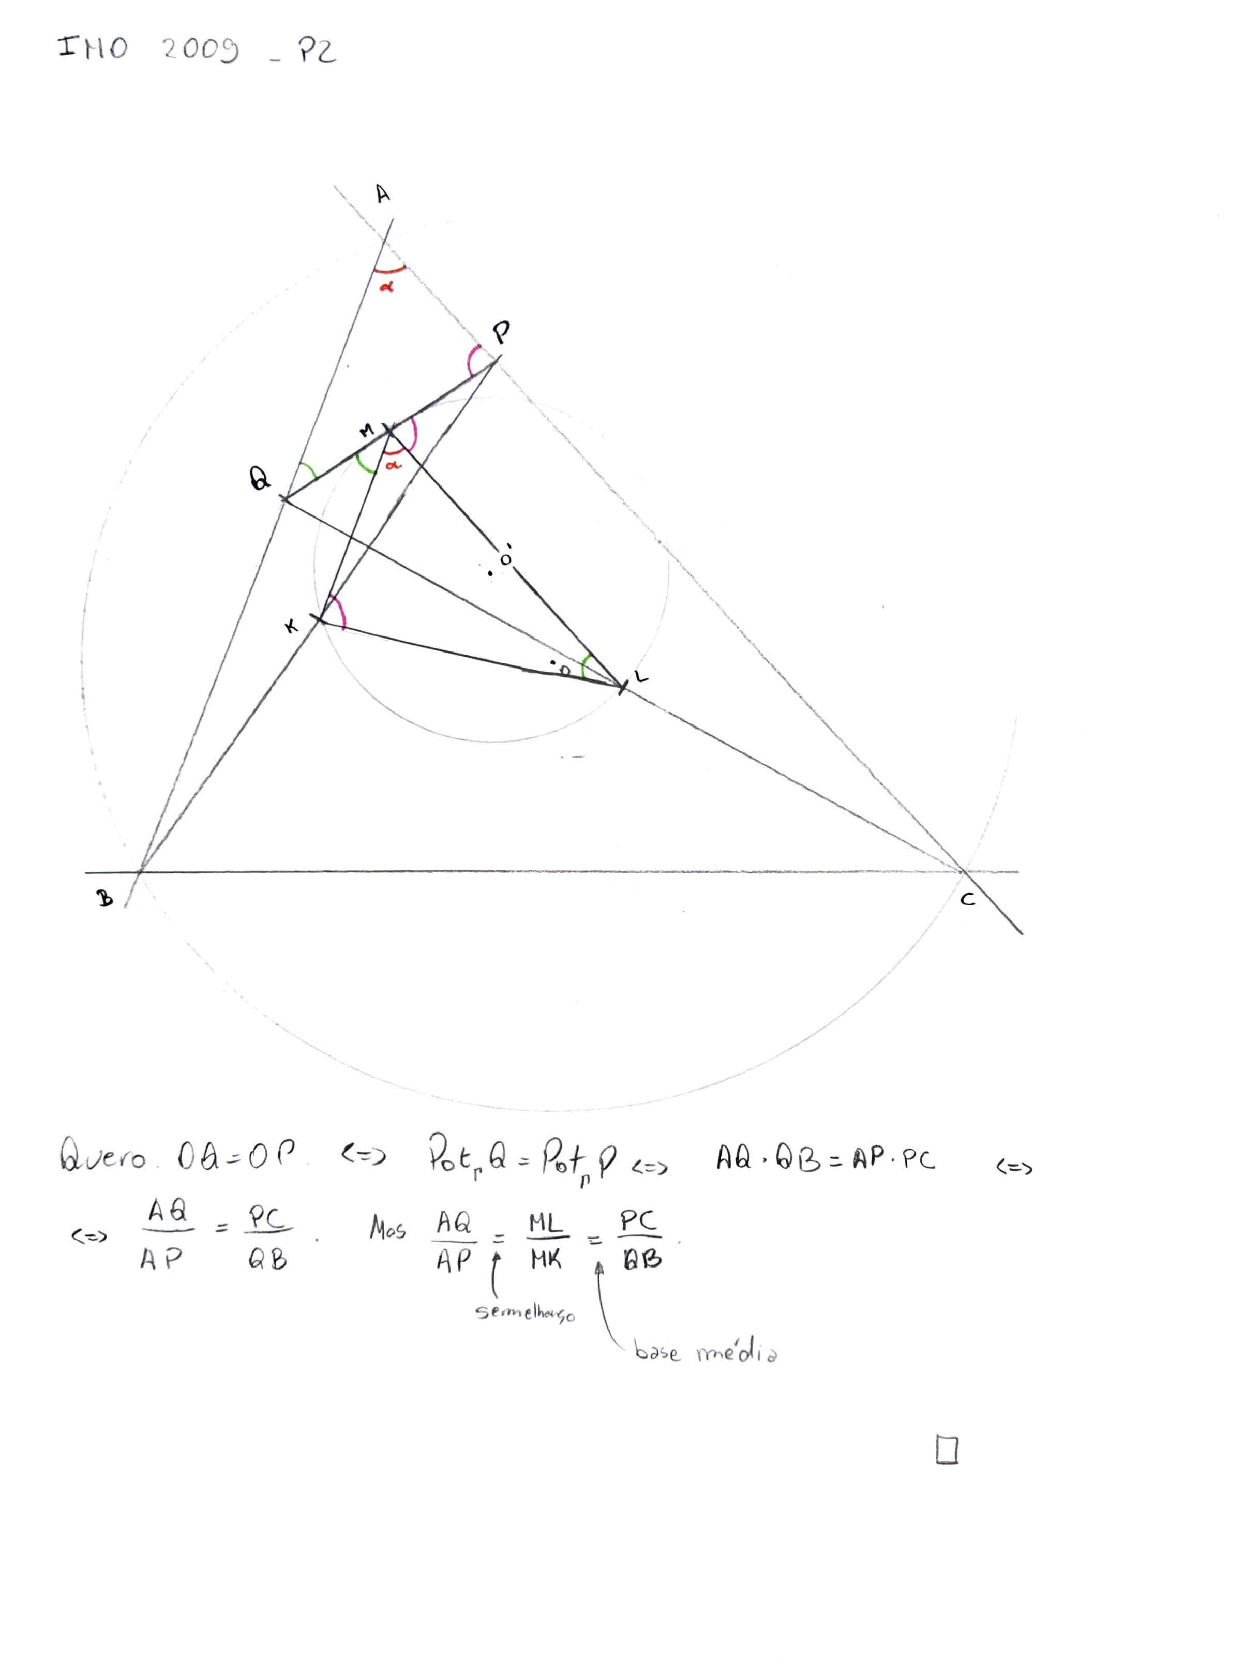
\includegraphics[width = 14cm]{/home/zeus/Documents/solutions/imo-2009-2''.pdf}

\newpage


% begin problem: egmo-2020-5 --lang en
\begin{prob}[EGMO 2020/5]
Consider the triangle $ABC$ with $\angle BCA > 90^{\circ}$. The circumcircle $\Gamma$ of $ABC$ has radius $R$. There is a point $P$ in the interior of the line segment $AB$ such that $PB = PC$ and the length of $PA$ is $R$. The perpendicular bisector of $PB$ intersects $\Gamma$ at the points $D$ and $E$.

Prove $P$ is the incentre of triangle $CDE$.
\end{prob}
% end problem

\newpage

% begin problem: imo-2014-3 --lang pt
\begin{prob}[IMO 2014/3]
Seja $ABCD$ um quadrilátero convexo com $\angle ABC = \angle CDA = 90^{\circ}$. O ponto $H$ é o pé da perperndicular de $A$ sobre $BD$. Os pontos $S$ e $T$ são escolhidos sobre os lados $AB$ e $AD$, respectivamente, de modo que $H$ esteja no interior do triângulo $SCT$ e \[ \angle CHS - \angle CSB = 90^{\circ}, \quad \angle THC - \angle DTC = 90^{\circ}. \]

Prove que a reta $BD$ é tangente à circunferência circunscrita ao triângulo $TSH$.
\end{prob}
% end problem

\newpage

% begin problem: imo-2008-1 --lang pt
\begin{prob}[IMO 2008/1]
Seja $H$ o ortocentro do triângulo acutângulo $ABC$. O círculo $\Gamma_{A}$, centrado no ponto médio de $BC$ que passa por $H$ intersecta a reta $BC$ nos pontos $A_{1}$ e $A_{2}$. Da mesma maneira, defina os pontos $B_{1}$, $B_{2}$, $C_{1}$ e $C_{2}$.

Prove que os seis pontos $A_{1}$, $ A_{2}$, $ B_{1}$, $ B_{2}$, $ C_{1}$ e $ C_{2}$ são concíclicos.
\end{prob}
% end problem



\end{document}
